\documentclass{article}
\usepackage{tabularx}
\usepackage{amsmath}
\usepackage{amssymb}
\usepackage{tikz}
\usetikzlibrary{timeline}
\usepackage{booktabs}
\usepackage{float}
\restylefloat{table}
\graphicspath{ {../} }
\usepackage[margin={1.5cm,2cm}]{geometry}
\usepackage{multicol}
\setlength\columnsep{1.5cm}
\usepackage{tabto}
\usepackage{pdflscape}
\usepackage{graphicx}
\usepackage{array}

\begin{document}
\begin{titlepage}
	\centering
	\begin{figure}[H]
	\centering
	%\includegraphics[scale=0.5]{logo_nasa_trio_black@2x.png}
	\end{figure}
	\vspace{2cm}
	{\scshape\LARGE NCRA-TIFR Project Proposal \par}
	\vspace{2cm}
	{\huge\bfseries \par}
	\vspace{2cm}
	{\Large\itshape Archit Sakhadeo\par}
	{\Large\itshape Rathin Desai\par}
	{\Large\itshape Shadab Shaikh\par}
	{\Large\itshape Shubhankar Deshpande\par}
	\vfill
	Mentor\par
	Dr. Yogesh  \textsc{Wadadekar}
	\par
	Dr. C. H. Ishwar \textsc{Chandra}

	\vfill

\end{titlepage}
\begin{multicols*}{2}
\section{Introduction}
\subsection{Morphological Classes of Radio Galaxies}

Radio galaxies with active nuclei can be distinguished based on their radio luminosity or brightness of their radio emissions in relation to their hosting environment. Some of the basic morphological classifications include point sources, extended sources i.e. sources with extended contours, double radio sources, jets, and lobes.


\subsection{Problems faced with current classification}

Currently Radio astronomers manually classify galaxies based on visual inspection of the images which is a slow procedure, and increases the time to production of scientific results. Further, it introduces uncertainities in the classification procedure, both of which are problems which can potentially be mitigated by using an automated approach.

Contemporary algorithms classify radio sources into at most three different classes. Our aim is to build a robust model capable of handling more than 2 classes.

\section{Objective}

\begin{itemize}
	\item Potentially discovering rare forms of radio sources by classification in different classes.
	\item Reduction in time to generate scientific results by radio astronomers.
	\item Deeper insight into topological representation of radio data during classification.
\end{itemize}

\section{Approach}

\subsection{Source Modelling}
  The first step would be source extraction using the standard technique of gaussian modelling. We propose to do this using the robust PyBDSM pipeline used for fitting gaussian distributions to radio sources. The software contains a plethora of features, from which we would be using a small subset. This would mainly include:

\begin{enumerate}
\item Source extraction using gaussian modelling of radio data.
\item Generation of a catalog file containing details of radio sources (RA, DEC, Size of Gaussian (min, max), etc.)
\end{enumerate}

\subsection{Cutout Generation}
The second step would be to convert the RA(Right Ascension) and DEC (Declination) values generated from the catalog, to their corresponding pixel values in the original image. Based on these pixel values we generate 10*10 px cutouts using as reference the co-ordinates of the center of the radio source. This involves a multistep procedure briefly including:
\begin{enumerate}
\item Using the astropy module to read the FITS image in the form of a matrix
\item Parsing through the generated catalog file using Pandas, and extracting data for each radio source such as RA, DEC, etc.
\item Converting the RA, DEC values using in-built functions in astropy to convert from WCS to pixel values.
\item Processing pixel values to account for difference in addressing between FORTRAN and C family of languages.
\item Slicing the image matrix assuming the reference pixel co-ordinates as the center of the source.
\item Storing the generated image cutout in a standard image format (JPEG), with name as (RA,DEC) values. 
\end{enumerate}

Prototype code for section \textit{3.1} and section \textit{3.2} has been written mainly for testing purposes. We used a sample image from the TGSS survey which was then processed using the first two steps of our pipeline to generate 470 cutout images.
More details may be found at: 
https://github.com/NCRA-TIFR/radiogen.

\subsection{Data Preprocessing}

Real world data are incomplete, inconsistent and noisy. Techniques like Data cleaning, integration, transformation, reduction, discretization are required to structure the data uniformly throughout the dataset in the required format.

Some regular techniques are:
\begin{itemize}


\item Mean subtraction 

It involves subtracting the mean across every individual feature in the data, and has the geometric interpretation of centering the cloud of data around the origin along every dimension.

\item Normalization

Normalization refers to normalizing the data dimensions so that they are of approximately the same scale. There are two common ways of achieving this normalization. One is to divide each dimension by its standard deviation, once it has been zero-centered. Another form of this preprocessing normalizes each dimension so that the min and max along the dimension is -1 and 1 respectively. 
\end{itemize}
\begin{figure}[H]
\centering
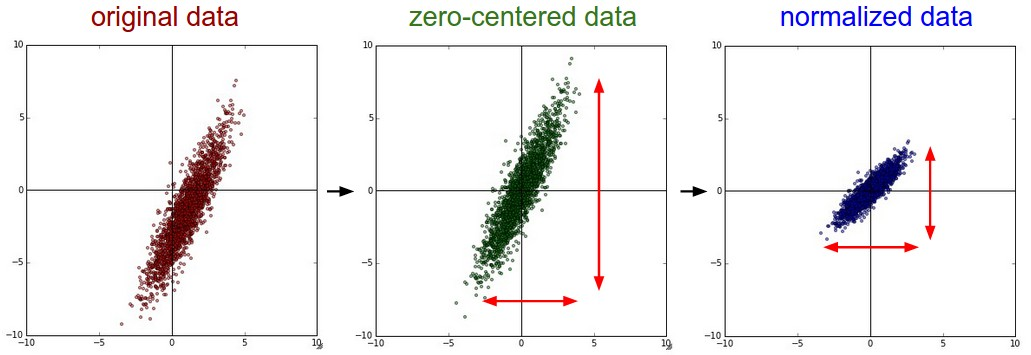
\includegraphics[scale=0.26]{prepro1.jpeg}
\caption{Mean Subtraction and Normalization}
\end{figure}
\begin{itemize}
\item Dimensionality reduction using Principal Component Analysis

The main linear technique for dimensionality reduction, principal component analysis, performs a linear mapping of the data to a lower-dimensional space in such a way that the variance of the data in the low-dimensional representation is maximized. By finding the eigen vector with the highest eigen value we select the Principal component axis with the highest variance and the minimum reconstruction error. Thus we reduce the dimensions by eliminating Principal component axes with the eigen vectors with the least variance thereby not losing much information.
\end{itemize}
\begin{figure}[H]
\centering
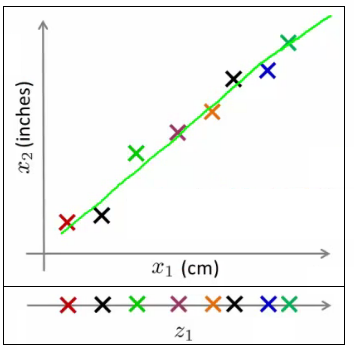
\includegraphics[scale=0.75]{pca.png}
\caption{Reduction from 2D to 1D using PCA}
\end{figure}
\subsection{Analytical Approach}

Some approaches that we plan to use: 
\begin{itemize}
\item Scale Invariant Feature Transform (SIFT

Statistical modelling of data to manually extract features. For any object in an image, interesting points on the object can be extracted to provide a "feature description" of the object. This description, extracted from a training image, can then be used to identify the object when attempting to locate the object in a test image containing many other objects. To perform reliable recognition, it is important that the features extracted from the training image be detectable even under changes in image scale, noise and illumination. SIFT is invariant of scaling, transformation and rotation.

\item Edge Detection

1) Reduction of noise using a Gaussian filter
2) Finding gradients along the X and Y directions in the image
3) Suppression of local minima
4) Double Thresholing to determine probable edges
5) Suppression of all weak edges which lack connection
\begin{figure}[H]
\centering
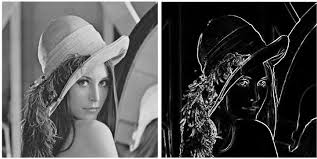
\includegraphics[scale=0.5]{edge.jpeg}
\caption{Edge detection}
\end{figure}


\item Image Segmentation

Image Segmentation is the process of partitioning a digital image into multiple segments. The goal of segmentation is to simplify and change the representation of an image into something that is more meaningful and easier to analyze. It is typically used to locate objects and boundaries (lines, curves, etc.) in images. More precisely, image segmentation is the process of assigning a label to every pixel in an image such that pixels with the same label share certain characteristics.
\end{itemize}
\begin{figure}[H]
\centering
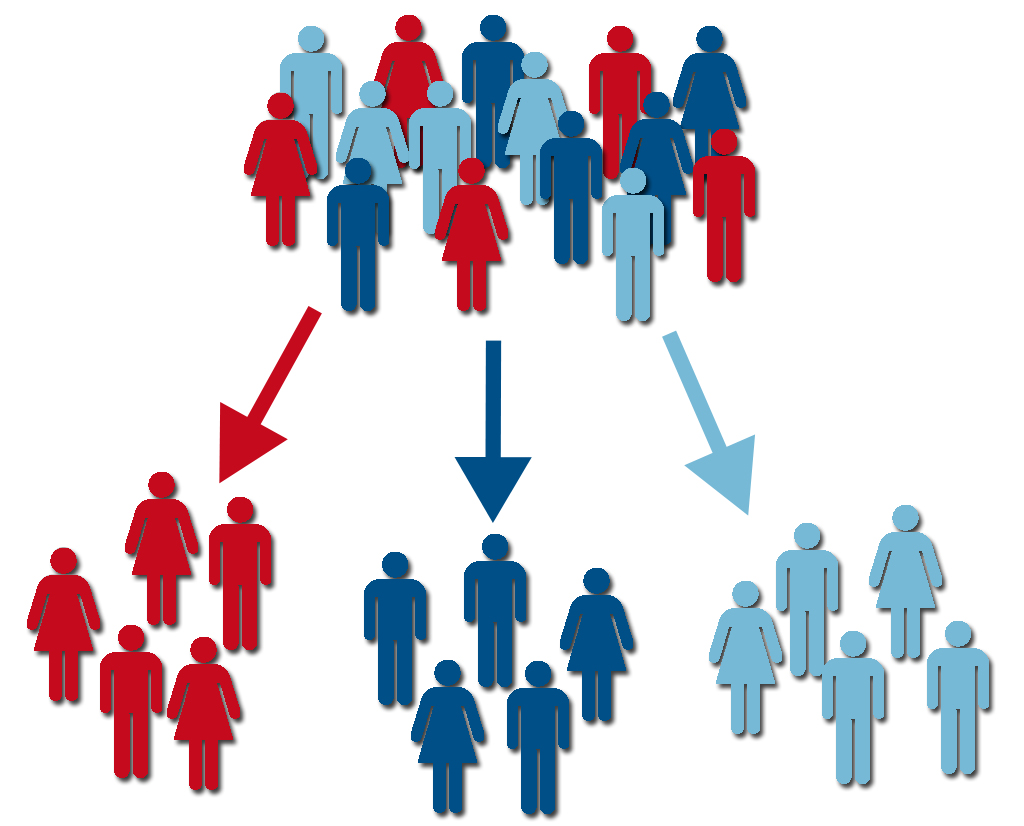
\includegraphics[scale=0.1]{segmentation.jpg}
\caption{Segmentation of data into distinct characteristics}
\end{figure}


\subsection{Empirical Approach}

We plan to deploy a Convolutional Neural Network model for classification which reduces the manual feature engineering part, and has achieved significant successes in object recognition and image classification tasks. ( Give References to papers) 
    


\section{How we predict it will solve the problem}

\section{Timeline}
\begin{itemize}
	\item 26th April to 11th May - literature survey
	\item Mid-August to October - working on basic prototype model individually by trying out multiple approaches
	\item October to November - choosing the approaches which work, and implementing them on all data, validation of the results.
	\item November to December - Refining the system, cleaning and commenting the code
\end{itemize} 





\section{Conclusion}
We would like to thank Dr.Yogesh Wadadekar \footnote{\label{NCRA-TIFR} National Center for Radio Astrophysics - Tata Institute of Fundamental Research}, Dr.C. H. Ishwara Chandra \footnotemark[\ref{NCRA-TIFR}] for their supportive presence during the process of brainstorming potential research ideas. Their constant guidance has been an invaluable source of inspiration for us, and we are eager to continue working with them.

\end{multicols*}
\end{document}
